%%
%% For submission/review: [acmsmall,screen,review]
%% For camera-ready:      [acmsmall]
%%
\documentclass[acmsmall,screen,review]{acmart}

%%
%% Author-year citations required by ACM TOMS.
%% Must appear in the preamble, before \begin{document}.
%%
\citestyle{acmauthoryear}

%%
%% Packages approved by ACM TAPS not already included in acmart.
%% Do NOT re-add: amsmath, booktabs, fontenc, inputenc, natbib,
%%                geometry, graphicx, hyperref, microtype, xcolor.
%%
\usepackage{algorithm}
\usepackage{algpseudocode}

%%
%% Rights management — replace with values from the ACM rights form.
%%
\setcopyright{acmlicensed}
\copyrightyear{2026}
\acmYear{2026}
\acmDOI{XXXXXXX.XXXXXXX}

\acmJournal{TOMS}
\acmVolume{0}
\acmNumber{0}
\acmArticle{0}
\acmMonth{0}

%%
%% end of preamble
%%
\begin{document}

\title{pysib: A Python Toolbox for System Identification}

\author{Diego Eckhard}
\affiliation{%
  \institution{Universidade Federal do Rio Grande do Sul}
  \city{Porto Alegre}
  \country{Brazil}
}
\email{diegoeck@ufrgs.br}
\orcid{0000-0001-8557-0384}

\renewcommand{\shortauthors}{Eckhard}

\begin{abstract}
\texttt{pysib} is an open-source Python package for parameter identification
of discrete-time SISO systems described by polynomial input--output model
structures.  It implements classical estimators for ARX, Stieglitz--McBride,
instrumental-variable, correlation, output-error, ARMAX, and Box--Jenkins
models.  All routines share a unified interface and a common polynomial
dictionary convention, so models estimated by different algorithms can be
evaluated through the same prediction and simulation functions.  Linear
estimators are implemented in Python using NumPy and SciPy.  The nonlinear
prediction-error estimators use a specialized conservative optimization core
for OE, ARMAX, and Box--Jenkins structures.  This optimizer deliberately uses
many small parameter updates, rather than relying on a few large steps, to
obtain a more controlled search trajectory on non-convex criteria.  The
large number of error, gradient, and sensitivity evaluations required by this
strategy is made practical by compiled C extensions and LAPACK routines for
the Gauss--Newton step.  The package also provides open implementations of
filtered continuation methods for the nonlinear estimators, progressively
relaxing data filters across optimization stages to reduce sensitivity to
local minima.
Monte Carlo experiments show that the SM and OE estimates are
centered close to the true parameters under additive output noise,
and that filtered continuation raises the empirical success rate of
the OE estimator from $60\,\%$ to $100\,\%$ on a non-convex
identification problem.
\end{abstract}

%%
%% CCS concepts — generate the correct codes at https://dl.acm.org/ccs/ccs.cfm
%%
\begin{CCSXML}
<ccs2012>
  <concept>
    <concept_id>10010147.10010169.10010170</concept_id>
    <concept_desc>Computing methodologies~Simulation and modeling</concept_desc>
    <concept_significance>500</concept_significance>
  </concept>
  <concept>
    <concept_id>10002950.10003705.10003707</concept_id>
    <concept_desc>Mathematics of computing~Mathematical software</concept_desc>
    <concept_significance>300</concept_significance>
  </concept>
</ccs2012>
\end{CCSXML}
\ccsdesc[500]{Mathematics of computing~Mathematical software}
\ccsdesc[300]{Computing methodologies~Simulation and modeling}

\keywords{system identification, Python, prediction-error method,
polynomial models, mathematical software}

\maketitle

\section{Introduction}
\label{sec:introduction}

Identifying dynamic models from measured input--output records is a
central problem in control, simulation, and signal processing.
Among the available model classes, discrete-time polynomial
input--output structures---ARX, ARMAX, output-error, and
Box--Jenkins---remain widely used because they are interpretable,
compact, and well supported by the prediction-error
framework~\cite{ljung1999,soderstrom1989}.
Estimating such models from data requires solving linear or nonlinear
least-squares problems, and for the nonlinear structures the quality
of the estimates also depends on initialization and the
optimization trajectory.

The MATLAB System Identification Toolbox and the SIB toolbox provide
mature, feature-rich implementations of these classical estimators,
but they are either proprietary or tied to a commercial
platform~\cite{mathworks_sysid,sib_matlab}.
In the open Python ecosystem, the SIPPY package offers a broad
collection of input--output and state-space routines~\cite{sippy},
while SysIdentPy focuses on nonlinear autoregressive models with
exogenous inputs~\cite{sysidentpy}.
A gap remains for an open-source Python package that is specifically
designed for polynomial prediction-error structures, with a specialized
optimization core and a unified model convention that allows
seamless switching between estimators.

\texttt{pysib} fills this gap.
It implements the main classical estimators---ARX, Stieglitz--McBride,
instrumental variables, correlation error minimization, output error,
ARMAX, and Box--Jenkins---together with prediction and simulation
routines that share a common polynomial dictionary (keys
\texttt{A}, \texttt{B}, \texttt{C}, \texttt{D}, \texttt{F}).
Linear estimators are written in Python with NumPy and SciPy; the
nonlinear prediction-error methods use compiled C extensions that
interface with LAPACK for the Newton step.
Filtered variants of the nonlinear estimators implement a continuation
strategy that makes the optimization less sensitive to local minima.

The package makes three contributions whose combination distinguishes
it from existing Python tools.
First, it is a focused, open-source, and well-tested toolbox for
polynomial input--output structures, with a simple API and a layered
Python/C architecture.
Second, the nonlinear OE, ARMAX, and BJ estimators employ a
conservative two-phase optimizer that deliberately uses many small
parameter updates rather than a few aggressive steps; the resulting
computational cost of repeated cost, gradient, and sensitivity
evaluations is made practical by compiled C extensions and LAPACK
linear solvers.
Third, \texttt{pysib} provides open implementations of filtered
continuation methods~\cite{eckhard2013input,eckhard2017cost} for the
nonlinear estimators; these methods progressively relax data filters
to drive the estimate toward the original PEM criterion; their
effect is evaluated below on a non-convex OE problem.

The remainder of the article is organized as follows.
Section~\ref{sec:problem-model-classes} defines the prediction-error
problem and the four polynomial model structures.
Section~\ref{sec:algorithms} describes the linear and nonlinear
estimators, the specialized optimization core, and the filtered
continuation strategy.
Section~\ref{sec:software-organization} outlines the software
architecture and the unified model convention.
Section~\ref{sec:numerical-results} presents Monte Carlo experiments
under noisy data and a study of the filtered continuation strategy
on a non-convex output-error problem.
Section~\ref{sec:conclusion} concludes the article.

\section{Problem and Model Classes}
\label{sec:problem-model-classes}

\subsection{The Identification Problem}
\label{subsec:identification-problem}

Consider a discrete-time single-input single-output (SISO) dynamical system
whose internal structure is unknown.  The system is driven by an input
$u(t) \in \mathbb{R}$ and produces a true output $y_0(t) \in \mathbb{R}$,
where $t$ indexes discrete-time samples.  The relationship is dynamic:
$y_0(t)$ depends on the current and past values of $u$, and possibly on past
values of the output itself.

An identification experiment applies an input signal $u(t)$ to the system for
$N$ time steps.  The output is not measured exactly; what is recorded is
\begin{equation}
    y(t) = y_0(t) + v(t), \qquad t = 1, \ldots, N,
    \label{eq:noisy-output}
\end{equation}
where $v(t)$ is an additive disturbance.  No specific structure is assumed for
$v(t)$ at this stage.

The identification problem is: given the data record
$\mathcal{D}_N = \{u(t),\,y(t)\}_{t=1}^{N}$, determine a parametric model
$\hat{y}(t;\theta)$---a function of past inputs and outputs, indexed by a
finite-dimensional parameter vector $\theta$---such that the prediction errors
$\varepsilon(t;\theta) = y(t) - \hat{y}(t;\theta)$ are small in a well-defined
sense.  The choice of model structure and the criterion for ``small'' are the
subjects of the following sections.

\subsection{Model Parameterization}
\label{subsec:model-structures}

The unknown system is parameterized by the general polynomial model
\begin{equation}
    y(t;\theta) = \frac{B(q^{-1};\theta)}{A(q^{-1};\theta)\,F(q^{-1};\theta)}\,u(t-n_k)
           + \frac{C(q^{-1};\theta)}{A(q^{-1};\theta)\,D(q^{-1};\theta)}\,e(t),
    \label{eq:general-model}
\end{equation}
where $\theta$ is the vector of free polynomial coefficients to be estimated,
$e(t)$ is a zero-mean white-noise sequence, $q^{-1}$ is the
backward-shift operator ($q^{-1}x(t) = x(t-1)$),
and $n_k \geq 0$ is the input delay in samples.
The polynomials are monic and defined in non-negative powers of $q^{-1}$:
\begin{align*}
    A(q^{-1};\theta) &= 1 + a_1 q^{-1} + \cdots + a_{n_a} q^{-n_a}, \\
    B(q^{-1};\theta) &= b_0 + b_1 q^{-1} + \cdots + b_{n_b-1}q^{-(n_b-1)}, \\
    C(q^{-1};\theta) &= 1 + c_1 q^{-1} + \cdots + c_{n_c} q^{-n_c}, \\
    D(q^{-1};\theta) &= 1 + d_1 q^{-1} + \cdots + d_{n_d} q^{-n_d}, \\
    F(q^{-1};\theta) &= 1 + f_1 q^{-1} + \cdots + f_{n_f} q^{-n_f}.
\end{align*}
For a given model structure, $\theta$ contains the coefficients of the
\emph{free} polynomials only (those not fixed to unity).  For example, for
the BJ structure all five polynomials contribute free coefficients, so
$\theta = [b_0,\ldots,b_{n_b-1},\,c_1,\ldots,c_{n_c},\,
           d_1,\ldots,d_{n_d},\,f_1,\ldots,f_{n_f}]^\top$;
for ARX, only $A$ and $B$ are free, giving
$\theta = [a_1,\ldots,a_{n_a},\,b_0,\ldots,b_{n_b-1}]^\top$.
The dimension $n_\theta$ depends on the chosen orders and structure.
The four standard structures are special cases of~\eqref{eq:general-model}
obtained by fixing some polynomials to unity, as listed in
Table~\ref{tab:structures}.
The plant transfer function and noise model are, respectively,
\begin{equation}
    G(q^{-1};\theta) = \frac{B(q^{-1};\theta)}{A(q^{-1};\theta)\,F(q^{-1};\theta)},
    \qquad
    H(q^{-1};\theta) = \frac{C(q^{-1};\theta)}{A(q^{-1};\theta)\,D(q^{-1};\theta)},
    \label{eq:gh}
\end{equation}
so~\eqref{eq:general-model} reads compactly as
$y(t;\theta) = G(q^{-1};\theta)\,u(t-n_k) + H(q^{-1};\theta)\,e(t)$.
At the true parameter vector $\theta_0$ this gives
$y_0(t) = G(q^{-1};\theta_0)\,u(t-n_k)$ and
$v(t) = H(q^{-1};\theta_0)\,e(t)$, making precise the
decomposition~\eqref{eq:noisy-output} of
Section~\ref{subsec:identification-problem}.
A key structural distinction
separates the four models: in ARX and ARMAX, the plant denominator and the
noise model share the same polynomial $A$, so the dynamics of the noise
and the plant are coupled; in OE and Box--Jenkins, the plant denominator
$F$ and the noise model $C/D$ are independent, allowing the two components
to be parameterized separately.

\begin{table}[t]
    \caption{Polynomial model structures supported by \texttt{pysib}.
             A free polynomial is estimated from data; a fixed polynomial
             is set to unity.}
    \label{tab:structures}
    \centering
    \footnotesize
    \setlength{\tabcolsep}{4pt}
    \begin{tabular}{lcccccc}
        \toprule
        Structure & $A$ & $B$ & $C$ & $D$ & $F$ & Noise model $H$ \\
        \midrule
        ARX   & free & free & $1$ & $1$ & $1$ & $1/A$ \\
        ARMAX & free & free & free & $1$ & $1$ & $C/A$ \\
        OE    & $1$  & free & $1$ & $1$ & free & $1$ \\
        BJ    & $1$  & free & free & free & free & $C/D$ \\
        \bottomrule
    \end{tabular}
\end{table}

Given the polynomial assignments in Table~\ref{tab:structures}, the
one-step-ahead predictor for the general structure~\eqref{eq:general-model} is
\begin{equation}
    \hat{y}(t \mid t-1;\theta) =
    y(t) + H(q^{-1};\theta)^{-1}
    \bigl[G(q^{-1};\theta)\,u(t-n_k) - y(t)\bigr],
    \label{eq:predictor}
\end{equation}
where $H(q^{-1};\theta)^{-1} = A(q^{-1};\theta)D(q^{-1};\theta)/C(q^{-1};\theta)$.
Substituting the structure assignments into~\eqref{eq:predictor} yields the
structure-specific predictor.  For the ARX structure,
\begin{equation}
    \hat{y}(t \mid t-1;\theta) =
    \sum_{j=0}^{n_b-1} b_j\,u(t-n_k-j)
    - \sum_{i=1}^{n_a} a_i\,y(t-i),
    \label{eq:arx-predictor}
\end{equation}
which is linear in $\theta$.
For the OE, ARMAX, and Box--Jenkins structures:
\begin{align}
    \hat{y}(t \mid t-1;\theta) &= \frac{B(q^{-1};\theta)}{F(q^{-1};\theta)}\,u(t-n_k),
    && \text{OE}, \label{eq:oe-predictor}\\
    \hat{y}(t \mid t-1;\theta) &= \frac{B(q^{-1};\theta)}{C(q^{-1};\theta)}\,u(t-n_k)
    + \frac{C(q^{-1};\theta)-A(q^{-1};\theta)}{C(q^{-1};\theta)}\,y(t),
    && \text{ARMAX}, \label{eq:armax-predictor}\\
    \hat{y}(t \mid t-1;\theta) &= y(t)
    + \frac{D(q^{-1};\theta)}{C(q^{-1};\theta)}
    \left[\frac{B(q^{-1};\theta)}{F(q^{-1};\theta)}\,u(t-n_k) - y(t)\right],
    && \text{BJ}. \label{eq:bj-predictor}
\end{align}
Thus, for Box--Jenkins models, prediction is evaluated by filtering the
plant-output mismatch through the inverse noise model $D(q^{-1};\theta)/C(q^{-1};\theta)$
and adding the result to the measured output.

\subsection{Parameter Estimation}
\label{subsec:criterion}

The prediction-error method (PEM) estimates $\theta$ by minimizing
the mean squared prediction error~\cite{ljung1999,soderstrom1989}
\begin{equation}
    V(\theta) = \frac{1}{N}\sum_{t=1}^{N} \varepsilon(t;\theta)^2,
    \label{eq:criterion}
\end{equation}
where $\varepsilon(t;\theta) = y(t) - \hat{y}(t \mid t-1;\theta)$ is the
one-step-ahead prediction error.
For the ARX predictor~\eqref{eq:arx-predictor}, writing
$\hat{y}(t \mid t-1;\theta) = \varphi(t)^\top\theta$ with the regression vector
\begin{equation}
  \varphi(t) = \bigl[-y(t-1),\ldots,-y(t-n_a),\,
                      u(t-n_k),\ldots,u(t-n_k-n_b+1)\bigr]^\top,
  \label{eq:regressor}
\end{equation}
and stacking $N$ rows into $\Phi \in \mathbb{R}^{N \times (n_a+n_b)}$ gives
$V(\theta) \propto \|\Phi\theta - y\|^2$,
whose minimum is the ordinary least-squares (OLS) solution
$\hat{\theta} = (\Phi^\top\Phi)^{-1}\Phi^\top y$.

The gradient of~\eqref{eq:criterion} with respect to $\theta$ is
determined by the \emph{sensitivity matrix}
$\Psi(\theta) \in \mathbb{R}^{N \times n_\theta}$, whose $j$-th column collects
\begin{equation}
  \psi_j(t;\theta) = \frac{\partial\hat{y}(t \mid t-1;\theta)}{\partial\theta_j}.
  \label{eq:sensitivity}
\end{equation}
Since $\varepsilon(t;\theta) = y(t) - \hat{y}(t \mid t-1;\theta)$, the chain rule gives
\begin{equation}
  \frac{\partial V}{\partial\theta} = -\frac{2}{N}\,\Psi(\theta)^\top\varepsilon(\theta),
  \label{eq:gradient-v}
\end{equation}
where $\varepsilon(\theta) = [\varepsilon(1;\theta),\ldots,\varepsilon(N;\theta)]^\top$.
For the ARX structure, $\psi_j(t;\theta) = \varphi_j(t)$ (the $j$-th entry of
the regression vector~\eqref{eq:regressor}), and~\eqref{eq:gradient-v} vanishes
exactly at the OLS solution.  For the OE, ARMAX, and Box--Jenkins structures, $\psi_j$
requires filtering through $1/F(q^{-1})$ or $1/C(q^{-1})$---polynomials
that depend on $\theta$ itself---making $\Psi$ a nonlinear function of
$\theta$ and~\eqref{eq:criterion} non-convex in general; the existence
of multiple local minima for these structures is well
documented~\cite{eckhard2011global,eckhard2012pem}.  The
Gauss--Newton approximation to the Hessian,
\begin{equation}
  \frac{\partial^2 V}{\partial\theta^2} \approx \frac{2}{N}\,\Psi^\top\Psi,
  \label{eq:gn-hessian-fw}
\end{equation}
retains only the outer-product term (dropping second-order sensitivity
terms that vanish near the minimum).  It is symmetric positive semidefinite
by construction; when the sensitivity matrix $\Psi$ has full column rank
the Gram matrix $\Psi^\top\Psi$ becomes positive definite and the
Gauss--Newton direction is well defined and points downhill.
Under standard regularity conditions on the input and noise,
global minimizers of the PEM criterion are consistent when the
true system belongs to the model class~\cite{ljung1999};
the implemented nonlinear routines seek such minima through local
optimization, so the numerical outcome also depends on
initialization and the optimizer.

Three estimators in \texttt{pysib} identify an ARX-structure model without
minimizing $V(\theta)$, avoiding the iterative nonlinear optimization
altogether.

\paragraph{Stieglitz--McBride (SM).}
The SM method~\cite{stieglitz1965} approximates the OE solution by replacing the single nonlinear
problem with a sequence of linear ones.  At each iteration $k$, the current
denominator estimate $\hat{F}^{(k)}(q^{-1})$ is used to filter both signals:
$u_f(t) = u(t)/\hat{F}^{(k)}(q^{-1})$ and
$y_f(t) = y(t)/\hat{F}^{(k)}(q^{-1})$.
An ARX model is then estimated on the filtered pair $(u_f, y_f)$,
and the new $\hat{F}^{(k+1)}$ is taken from the feedback polynomial of that
ARX solution.  The procedure is repeated for a fixed number of iterations
(100 in \texttt{pysib}).  Although a fixed point of this iteration satisfies
the same normal equations as the OE solution, the method is not guaranteed to
reach the global minimum of $V(\theta)$~\cite{ljung1999}.

\paragraph{Instrumental Variables (IV).}
The IV method estimates an ARX model consistently even when the noise
is not of the form $1/A(q^{-1};\theta)\,e(t)$, at the cost of requiring two
independent experiments driven by the same input $u(t)$.  Let
$y_i(t) = y_0(t) + e_i(t)$, $i = 1,2$, denote the noisy outputs, where
$y_0(t)$ is the true plant output and $e_1(t)$, $e_2(t)$ are independent
noise sequences.  Define the regression matrix
$\Phi_1 \in \mathbb{R}^{N \times (n_a+n_b)}$ with rows
\[
  \varphi_1(t)^\top = \bigl[-y_1(t-1),\ldots,-y_1(t-n_a),\,
                             u(t-n_k),\ldots,u(t-n_k-n_b+1)\bigr],
\]
and the instrument matrix $Z \in \mathbb{R}^{N \times (n_a+n_b)}$ with rows
\[
  \zeta(t)^\top = \bigl[-y_2(t-1),\ldots,-y_2(t-n_a),\,
                         u(t-n_k),\ldots,u(t-n_k-n_b+1)\bigr],
\]
where the lagged $y_1$ entries of $\varphi_1$ are replaced by the
corresponding lagged $y_2$ entries.  The IV estimate is
\begin{equation}
    \hat{\theta} = (Z^\top \Phi_1)^{-1} Z^\top y_1.
    \label{eq:iv}
\end{equation}
Because $Z$ shares the input-driven part of $\Phi_1$ but $Z^\top e_1 \to 0$
as $N \to \infty$ (since $e_2$ and $e_1$ are independent),
$\hat{\theta}$ is consistent~\cite{soderstrom1989}.

\paragraph{Correlation method.}
The correlation method finds $\theta$ by requiring the prediction error
$\varepsilon(t;\theta)$ to be uncorrelated with an instrument $z(t)$ at
$M$ lags:
\begin{equation}
    \frac{1}{N}\sum_t z(t-\tau)\,\varepsilon(t;\theta) = 0,
    \qquad \tau = 0,1,\ldots,M-1.
    \label{eq:correlation}
\end{equation}
Since $\varepsilon(t;\theta)$ is linear in $\theta$ for the ARX structure,
\eqref{eq:correlation} constitutes a system of $M$ linear equations.
For $M = n_a + n_b$ the system is exactly determined; for $M > n_a + n_b$
it is overdetermined and solved by least squares, which minimizes the sum
of squared cross-correlations.  The default instrument is $z = u$, which
is valid in open-loop experiments where the input is uncorrelated with the
noise.

These three estimators serve a dual role in the package.  They can be
applied directly when their respective conditions are satisfied.  They also
provide the initial parameter vector for every nonlinear PEM estimator in
\texttt{pysib}: each nonlinear method is warm-started from an ARX solution,
so the iterative optimizer begins from a meaningful point rather than an
arbitrary initial guess.

\section{Algorithms}
\label{sec:algorithms}

\subsection{Linear Estimators}
\label{subsec:linear-estimators}

\subsubsection{ARX}
\label{subsubsec:arx}

The ARX estimator is the fundamental linear routine in the package and the
warm-start for every nonlinear method.
The ARX predictor~\eqref{eq:arx-predictor} is linear in $\theta$:
$\hat{y}(t \mid t-1;\theta) = \varphi(t)^\top\theta$,
where $\varphi(t)$ is the regression vector~\eqref{eq:regressor}.
Stacking $N$ rows into the regression matrix
$\Phi \in \mathbb{R}^{N \times n_\theta}$ and the outputs into
$y = [y(1),\ldots,y(N)]^\top \in \mathbb{R}^N$,
the PEM criterion~\eqref{eq:criterion} reduces to
\[
    V(\theta) = \frac{1}{N}\,\|\Phi\theta - y\|^2,
\]
which is a convex quadratic function of $\theta$ (the Hessian
$\frac{2}{N}\Phi^\top\Phi$ is positive semidefinite).
Differentiating and setting $\partial V/\partial\theta = 0$ yields the
\emph{normal equations}
\[
    \Phi^\top\Phi\,\hat\theta = \Phi^\top y.
\]
The solution is unique if and only if $\Phi$ has full column rank, i.e.,
$\Phi^\top\Phi$ is invertible, in which case
$\hat\theta = (\Phi^\top\Phi)^{-1}\Phi^\top y$ is the unique global
minimum of $V(\theta)$.  Full column rank is obtained in open-loop identification when the input
$u(t)$ is \emph{persistently exciting} of order $n_\theta$: informally,
the input must contain enough distinct frequency components to excite all
modes of the regression matrix~\cite{ljung1999}.  When this condition
fails (e.g., a constant or insufficiently rich input), $\Phi$ is
rank-deficient and $V(\theta)$ has infinitely many minimizers forming an
affine subspace.

Computing $(\Phi^\top\Phi)^{-1}$ directly is numerically inadvisable
even in the full-rank case: the condition number satisfies
$\kappa(\Phi^\top\Phi) = \kappa(\Phi)^2$, so any ill-conditioning in
$\Phi$ is squared, amplifying rounding errors.  \texttt{pysib} instead
calls \texttt{numpy.linalg.lstsq}, which invokes the LAPACK driver
\texttt{dgelsd}.  This routine solves the least-squares problem via the
divide-and-conquer SVD of $\Phi$ directly, avoiding the normal equations
entirely.  When $\Phi$ is rank-deficient, \texttt{dgelsd} returns the
minimum-norm solution among all minimizers of $V(\theta)$.

\subsubsection{Stieglitz--McBride}
\label{subsubsec:sm}

The OE predictor $\hat{y}(t \mid t-1;\theta) = B(q^{-1};\theta)/F(q^{-1};\theta)\,u(t-n_k)$
is nonlinear in the $F$ coefficients, making $V(\theta)$ non-convex.
The SM method approximates the OE solution by replacing the single
nonlinear problem with a sequence of linear ARX problems.

At each iteration $k$, the current denominator estimate
$\hat{F}^{(k)}(q^{-1};\theta)$ is used to prefilter both signals:
\[
  u_f(t) = \frac{u(t)}{\hat{F}^{(k)}(q^{-1};\theta)}, \qquad
  y_f(t) = \frac{y(t)}{\hat{F}^{(k)}(q^{-1};\theta)}.
\]
An ARX model of orders $(n_f, n_b)$ is then estimated on the filtered
pair $(u_f, y_f)$ using the procedure of Section~\ref{subsubsec:arx},
and the new denominator estimate $\hat{F}^{(k+1)}$ is taken from the
feedback polynomial of that ARX solution.
At a fixed point $\hat{F}^{(k+1)} = \hat{F}^{(k)}$, the ARX normal
equations on the filtered data reduce to the OE optimality conditions,
so the fixed point is an OE solution.  However, convergence to the
global minimum is not guaranteed~\cite{ljung1999}; the result depends
on the initialization.  \texttt{pysib} initializes $\hat{F}^{(0)}$
from a plain ARX solution on the unfiltered data.

\begin{algorithm}
\caption{Stieglitz--McBride}
\label{alg:sm}
\begin{algorithmic}[1]
\Require $u$, $y$, orders $n_b$, $n_f$, $n_k$, iterations $K=100$
\State $\hat{\theta} \leftarrow \texttt{arx}(u, y, n_f, n_b, n_k)$
       \Comment{ARX warm-start: $\hat{F}^{(0)}$ from $\hat{A}$}
\For{$k = 1, \ldots, K$}
  \State $u_f \leftarrow u \,/\, \hat{F}^{(k-1)}(q^{-1};\theta)$
  \State $y_f \leftarrow y \,/\, \hat{F}^{(k-1)}(q^{-1};\theta)$
  \State $\hat{\theta} \leftarrow \texttt{arx}(u_f, y_f, n_f, n_b, n_k)$
         \Comment{OLS on filtered pair}
  \State $\hat{F}^{(k)} \leftarrow \hat{A}$ from $\hat{\theta}$
\EndFor
\State \Return $\hat{\theta}$
\end{algorithmic}
\end{algorithm}

The IV and correlation estimators follow the constructions of
Section~\ref{subsec:criterion} and are implemented in Python using
NumPy.

\subsubsection{Instrumental Variables}
\label{subsubsec:iv}

The IV estimator solves the linear system
$(Z^\top\Phi_1)\,\hat\theta = Z^\top y_1$,
where $\Phi_1$ and $Z$ are the regression and instrument matrices
defined in Section~\ref{subsec:criterion}.
The system is solved by least squares via
\texttt{numpy.linalg.lstsq}.
The method requires two independent experiments driven by the same
input $u(t)$, and it is consistent when the noise sequences in the
two experiments are uncorrelated with each other and with the input.
In \texttt{pysib}, the IV routine accepts a single pair
$(u, y_1)$ and a second output record $y_2$; when the two outputs
are identical, the method reduces to ordinary least-squares ARX.

\subsubsection{Correlation}
\label{subsubsec:correlation}

The correlation estimator assembles the $M \times (n_a+n_b)$ matrix
of cross-correlations between the instrument $z(t)$ and the lagged
signals that appear in the ARX predictor.
The default instrument is $z = u$, which is valid in open-loop
experiments where the input is uncorrelated with the noise.
When $M = n_a + n_b$, the linear system~\eqref{eq:correlation}
is exactly determined; when $M > n_a + n_b$, it is overdetermined
and solved via \texttt{numpy.linalg.lstsq}, which finds the
least-squares solution that minimizes the sum of squared
cross-correlations.
The implementation follows the same pattern as ARX: the regressor
matrix is assembled once and the result returned without iteration.

\subsection{Nonlinear Prediction-Error Estimators and Optimization Core}
\label{subsec:nonlinear-optimization-core}

The OE, ARMAX, and Box--Jenkins estimators minimize the nonlinear
prediction-error criterion $V(\theta)$ using the
gradient~\eqref{eq:gradient-v} and the Gauss--Newton
Hessian~\eqref{eq:gn-hessian-fw}.  Since the filters in these structures
depend on the parameters, the resulting criteria are generally non-convex.
For this reason, \texttt{pysib} uses a specialized optimization core rather
than treating the estimators as generic black-box minimization problems.
The core combines structure-specific sensitivity recursions with a
conservative search strategy based on many small parameter updates, followed
by Gauss--Newton refinement.  This design increases the number of error,
gradient, and sensitivity evaluations, and the performance-critical routines
are therefore implemented as compiled C extensions; the Newton system is
solved through LAPACK.  Each estimator is initialized from an ARX solution;
noise-model polynomials ($C$, $D$) are initialized to zero free coefficients.

\paragraph{Structure-specific sensitivities.}
The nonlinear estimators use analytic, structure-specific sensitivity
recursions rather than numerical differentiation.  Separate C modules are
used for OE, ARMAX, and Box--Jenkins because the free polynomials and the
filters appearing in the sensitivity equations differ across structures.
For the OE predictor $\hat{y}(t) = B(q^{-1})/F(q^{-1})\,u(t-n_k)$,
for example, the sensitivities~\eqref{eq:sensitivity} are
\begin{align}
  \psi_{b_j}(t) &= \frac{q^{-j}\,u(t-n_k)}{F(q^{-1})},
                 \label{eq:sens-b} \\
  \psi_{f_j}(t) &= -\frac{q^{-j}\,\hat{y}(t)}{F(q^{-1})}.
                 \label{eq:sens-f}
\end{align}
For ARMAX the denominator filter is $1/C(q^{-1})$; for Box--Jenkins both
$1/F(q^{-1})$ and $1/C(q^{-1})$ appear, together with the corresponding
noise-model polynomials.  Thus each C module implements the sensitivity
recursions for its own polynomial structure.

\paragraph{Reuse of filtered sensitivity sequences.}
The C implementation also exploits the shift structure of polynomial
models.  Many sensitivity columns differ only by a delay.  In these cases,
the code first computes a filtered base sequence and then forms the
corresponding columns by time shifts, instead of applying the same IIR
filter separately for every coefficient.  In the OE case, a single pass
through $1/F(q^{-1})$ applied to the delayed input provides the base
sequence for all numerator sensitivities, while a single pass applied to
$-\hat{y}$ provides the base sequence for the denominator sensitivities;
the columns associated with $b_j$ and $f_j$ are obtained by indexing these
sequences with the appropriate lag.  The same principle is used in the
ARMAX and Box--Jenkins modules with their respective filters.  This reuse is
important because the optimizer evaluates the cost, gradient, and
Gauss--Newton matrices many times along a single identification run.

\paragraph{Selective cost, gradient, and Hessian evaluation.}
The optimization core distinguishes between three levels of computation.
When only a candidate parameter vector must be accepted or rejected, it
evaluates the cost $V(\theta)$ without forming sensitivities.  During the
initial descent phase, it evaluates the cost and gradient but does not build
the Gauss--Newton matrix.  During the Newton phase, it evaluates the cost,
gradient, and the matrix $\Psi^\top\Psi$ needed in
\eqref{eq:newton-system}.  This separation avoids unnecessary gradient or
Hessian assembly during the many small trial steps used by the optimizer.
For scalar cost comparisons the C core internally uses the
root-mean-square prediction error \smash{$\sqrt{V(\theta)}$}, which
does not change minimizers or accept/reject ordering because it is
strictly increasing in~$V$; the gradient and Gauss--Newton quantities
retain the standard least-squares scaling and are unaffected by a
constant factor in the cost.

\paragraph{Two-phase optimizer.}
\emph{Phase~1} is a conservative smoothed steepest-descent loop intended to
stabilize the trajectory from the ARX warm start before local Newton
refinement.  At each of up to $100 \times 100$ gradient evaluations, the
gradient $g = \partial V/\partial\theta$~\eqref{eq:gradient-v} is accumulated
by an exponential moving average, $d \leftarrow (4d + g)/5$, which damps
iteration-to-iteration changes in the descent direction.  The direction is
normalized to unit length, separating the direction of motion from the step
size, and the parameter vector is updated by
$\theta \leftarrow \theta - \alpha\,d/\|d\|$.  The step size $\alpha$ adapts
slowly and multiplicatively: $\alpha \leftarrow 1.01\,\alpha$ on a cost
decrease and $\alpha \leftarrow 0.99\,\alpha$ on an increase, starting from
$\alpha = 10^{-5}$.  The phase terminates early when $\alpha < 10^{-7}$.

\emph{Phase~2} performs local Gauss--Newton refinement using the structured
sensitivities computed by the C module.  At each of $1000$ iterations the
Newton direction $\delta$ is obtained by solving
\begin{equation}
  (\Psi^\top\Psi)\,\delta = -\Psi^\top\varepsilon
  \label{eq:newton-system}
\end{equation}
via the LAPACK routine \texttt{dposv}, which solves the Gauss--Newton
normal system by Cholesky factorization under the assumption of positive
definiteness.  The candidate
$\theta \leftarrow \theta - \alpha_k\,\delta$ uses a growing step
$\alpha_k = (k+1)/1000$, ranging from $0.002$ at the first iteration to
approximately $1$ at the last, so full Newton steps are approached gradually.
If the candidate does not reduce the cost or is non-finite, a bisection
safeguard is applied up to ten times:
$\theta^{\mathrm{new}} \leftarrow (\theta^{\mathrm{new}} + \theta)/2$.

\subsection{Filtered Continuation Estimators}
\label{subsec:filtered-continuation-estimators}

Nonlinear prediction-error criteria may have multiple local minima, and
even a conservative optimizer may converge to a nonglobal stationary point.
The filtered estimators in \texttt{pysib} provide open implementations of
the continuation and cost-function-shaping strategies developed for this
setting~\cite{eckhard2013input,eckhard2017cost}.  At each continuation
stage, filtering the input--output data modifies the shape of the cost
function; progressively relaxing the filter then drives the estimate toward
the original unfiltered criterion.  Filtered variants are provided for the
OE, ARMAX, and Box--Jenkins estimators; in each case the final stage
runs the corresponding unfiltered estimator on the original PEM criterion.

\paragraph{Stage sequence and warm-starting.}
The procedure runs nine filtered optimization stages followed by one
final stage on the unfiltered data.  Each stage calls the same nonlinear
optimization core used by the corresponding unfiltered estimator, but on a
filtered version of the input--output record.  The solution returned by one
stage is used as the initial condition for the next stage, so the
continuation path begins from a strongly shaped criterion and ends at the
original PEM problem.  The total computational cost is approximately ten
times that of the corresponding unfiltered estimator.

\paragraph{Filter schedules.}
For the OE structure, each stage uses a first-order IIR filter
$(1-a_i)/(1 - a_i q^{-1})$ with unit DC gain, whose pole is
$a_i = 0.05^{1/\tau_i}$ with $\tau_i = 4(10 - i)$ for stages
$i = 1,\ldots,9$.  The pole decreases from $a_1 \approx 0.920$
(aggressive low-pass, stage~1) to $a_9 \approx 0.473$ (mild
low-pass, stage~9), progressively restoring high-frequency content.

For the ARMAX and Box--Jenkins structures, each stage uses a
first-order Butterworth filter with normalized cutoff
$\omega_i = 0.1\,i$ (as a fraction of the Nyquist frequency),
$i = 1,\ldots,9$.  Stage~1 passes only the lowest $10\,\%$ of the
spectrum; stage~9 passes $90\,\%$.  In both schedules the final stage is the original unfiltered
estimator applied to the same PEM criterion; the only difference
between the standard and filtered methods is the initial
condition---the standard method starts from an ARX estimate,
while the filtered method starts from the solution of the
previous filtered stage.

The numerical experiments in
Section~\ref{sec:numerical-results} focus on the OE structure because
the theoretical analysis of cost-function shaping was developed
specifically for the output-error
case~\cite{eckhard2013input,eckhard2017cost}.
The same continuation strategy is implemented for ARMAX and
Box--Jenkins in \texttt{pysib} under the expectation that the mechanism
of progressively relaxing data filters should also improve convergence
in those structures, although formal guarantees have not been
established for them.

\section{Software Organization}
\label{sec:software-organization}

\paragraph{Python/C separation.}
The package separates Python-level orchestration from performance-critical
compiled routines.  Linear estimators (ARX, SM, IV, correlation) are
implemented in Python using NumPy and SciPy.  The nonlinear PEM optimizers
are compiled as three separate C extension modules
(\texttt{sib\_oe\_module.c}, \texttt{sib\_armax\_module.c},
\texttt{sib\_bj\_module.c}), each providing the structure-specific
sensitivity formulas and sharing the common two-phase optimizer from
\texttt{sib\_optimize.c}.  The Newton step in Phase~2 links against
LAPACK (\texttt{dposv}) without requiring an external system identification
framework.  The filtered variants are Python wrappers that sequence the
filter stages and delegate each optimization to the corresponding C module.

\paragraph{Unified model convention.}
Every estimation routine returns a pair $(\hat\theta, m)$.
The vector $\hat\theta$ contains the free parameter estimates in
structure-specific order, and the dictionary $m$ stores the polynomial
coefficient vectors under the keys \texttt{A}, \texttt{B}, \texttt{C},
\texttt{D}, and \texttt{F} (fixed polynomials contain only~$[1]$).
The \texttt{predict} and \texttt{simulate} routines share the same
dictionary convention, so any estimated model can be evaluated through
a common model representation.

\paragraph{Article/manual boundary.}
This article describes the algorithms and the high-level organization of
the software.  Installation instructions, dependency versions, complete API
documentation, callable-procedure examples, and expected driver outputs are
provided in the accompanying user manual, as required for the CALGO software
component.

Table~\ref{tab:architecture} summarizes the main components and their
implementations.

\begin{table}[t]
    \caption{Main software components of \texttt{pysib}.}
    \label{tab:architecture}
    \centering
    \footnotesize
    \setlength{\tabcolsep}{3pt}
    \begin{tabular}{p{0.30\columnwidth}p{0.30\columnwidth}p{0.27\columnwidth}}
        \toprule
        Component & Implementation & Role \\
        \midrule
        ARX, SM, IV, Correlation & Python, NumPy, SciPy & Linear estimators \\
        OE, ARMAX, BJ & C extension, LAPACK & Nonlinear prediction-error estimators \\
        Filtered variants & Python over C optimizer & Continuation strategy \\
        Prediction and simulation & SciPy \texttt{lfilter} & Model evaluation \\
        \bottomrule
    \end{tabular}
\end{table}

\section{Numerical Results}
\label{sec:numerical-results}

The accompanying software artifact includes deterministic unit tests for
noise-free exact recovery and for the polynomial convention of
Section~\ref{sec:problem-model-classes}.  These tests cover all public
estimators---ARX, SM, IV, correlation, OE, ARMAX,~BJ, and the filtered
variants---on low-order systems with known parameters.
They are part of the software validation and are not presented as
scientific results.  The numerical experiments reported here focus instead
on the behavior of the estimators under noisy data and on the effect of
filtered continuation in non-convex identification problems.

\subsection{Robustness under Noisy Data}
\label{subsec:robustness-noisy-data}

The first experiment evaluates the SM and OE estimators
under additive output noise; ARX is included only as a structurally
mismatched linear baseline.
A second-order OE system with true polynomials
$B(q^{-1}) = q^{-1}$ and
$F(q^{-1}) = 1 - 1.1q^{-1} + 0.2625q^{-2}$ is driven by a
three-sine input of length $N=500$.
White Gaussian noise with standard deviation $\sigma_v = 0.1$ is added
to the output, and $M=500$ independent realizations are used.
ARX is estimated with a structurally incorrect second-order linear
model; SM and OE use orders $(n_b,n_f,n_k) = (1,2,1)$ matching the
true plant.
Table~\ref{tab:robustness-params} reports the mean and
sample deviation of the OE-structure parameter estimates.
The SM and OE estimates are centered close to the true parameters,
with deviations below $5 \times 10^{-3}$.
(The notation $b_1$ refers to the first non-zero $B$ coefficient
after the delay $n_k=1$, following the definitions in
Section~\ref{sec:problem-model-classes}.)
Figure~\ref{fig:robustness-params} shows the corresponding
histograms per parameter.
ARX, with a mismatched noise structure, serves
as a linear baseline and is not directly comparable parameter-wise.
The corresponding simulation drivers and expected outputs are
included in the software artifact.

\begin{table}[t]
  \caption{Mean and standard deviation of the OE-structure parameter
           estimates under noisy data ($M=500$).}
  \label{tab:robustness-params}
  \centering
  \footnotesize
  \setlength{\tabcolsep}{4pt}
  \begin{tabular}{lcccc}
    \toprule
    Method & $b_1$ (true~$1$) & $f_1$ (true~$-1.1$) & $f_2$ (true~$0.2625$) \\
    \midrule
    SM & $1.0004 \pm 0.0044$ & $-1.0997 \pm 0.0038$ & $0.2623 \pm 0.0033$ \\
    OE & $1.0003 \pm 0.0044$ & $-1.0998 \pm 0.0038$ & $0.2623 \pm 0.0033$ \\
    \bottomrule
  \end{tabular}
\end{table}

\begin{figure}[t]
  \centering
  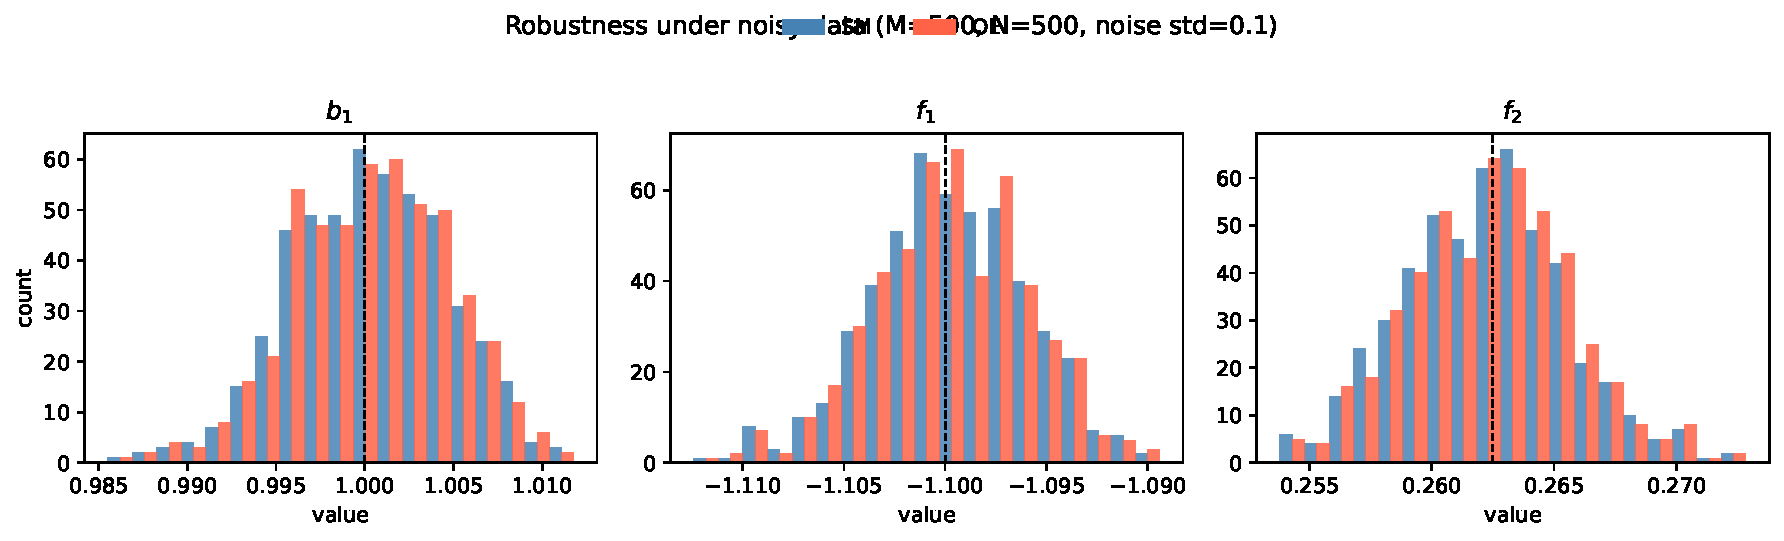
\includegraphics[width=\columnwidth]{experiments/robustness_noisy_data_parameters.pdf}
  \caption{Monte Carlo histograms of the OE-structure parameter estimates
           for SM and OE.
           Dashed vertical lines mark true values.}
  \Description{Three side-by-side histograms of the
    OE-structure parameter estimates (b1, f1, f2) comparing SM
    and OE distributions, with dashed vertical lines at the true
    parameter values.}
  \label{fig:robustness-params}
\end{figure}

\subsection{Effect of Filtered Continuation}
\label{subsec:filtered-continuation}

The second experiment tests whether the filtered continuation strategy
improves the convergence of the OE estimator when the PEM criterion
has multiple local minima.
The true system is a third-order OE plant with
$B(q^{-1}) = q^{-1}$ and
$F(q^{-1}) = 1 - 2.4q^{-1} + 1.91q^{-2} - 0.504q^{-3}$,
corresponding to poles at $0.9$, $0.8$, and $0.7$.
The input is a three-sine signal of length $N=1000$, and
white Gaussian noise with $\sigma_v = 30$ is added to the output,
yielding a signal-to-noise ratio of approximately $-6$\,dB.
A Monte Carlo of $M=100$ independent realizations is performed;
both estimators use ARX-based initializations and the same
optimization core
(Section~\ref{subsec:nonlinear-optimization-core}):
the standard OE method proceeds directly to the unfiltered
criterion, whereas the filtered variant first follows the filtered
continuation path before its final unfiltered stage.

Quality is measured by the relative simulation error
$\|y_0 - \hat{y}\|_2 / \|y_0\|_2$ on the noise-free output,
and a run is considered successful if this error is below~$5\,\%$,
a typical practical tolerance for model-based control applications.
Table~\ref{tab:filtered-results} reports the mean and standard deviation
of the error for both methods, as well as the success rate.
The standard OE estimator succeeds in $60\,\%$ of the Monte Carlo runs
(95\,\% Wilson confidence interval $[50\,\%,69\,\%]$),
with a mean error of $5.7 \times 10^{-2}$.
The filtered variant succeeds in $100\,\%$ of the runs and reduces the
mean error to $2.2 \times 10^{-2}$.
Figure~\ref{fig:filtered-errors} shows the error distribution and a
boxplot of both estimators.
The tenfold increase in computational cost due to the nine filtered
stages is the price paid for achieving a $100\,\%$ empirical success
rate in this problem.

\begin{table}[t]
  \caption{Relative simulation error of OE and OE filtered
           on a non-convex OE identification problem ($M=100$).}
  \label{tab:filtered-results}
  \centering
  \footnotesize
  \begin{tabular}{lccc}
    \toprule
    Method & Mean error & Std error & Success rate ($<5\%$) \\
    \midrule
    OE & $5.69 \times 10^{-2}$ & $4.37 \times 10^{-2}$ & $60\%$ \\
    OE filtered & $2.17 \times 10^{-2}$ & $7.94 \times 10^{-3}$ & $100\%$ \\
    \bottomrule
  \end{tabular}
\end{table}

\begin{figure}[t]
  \centering
  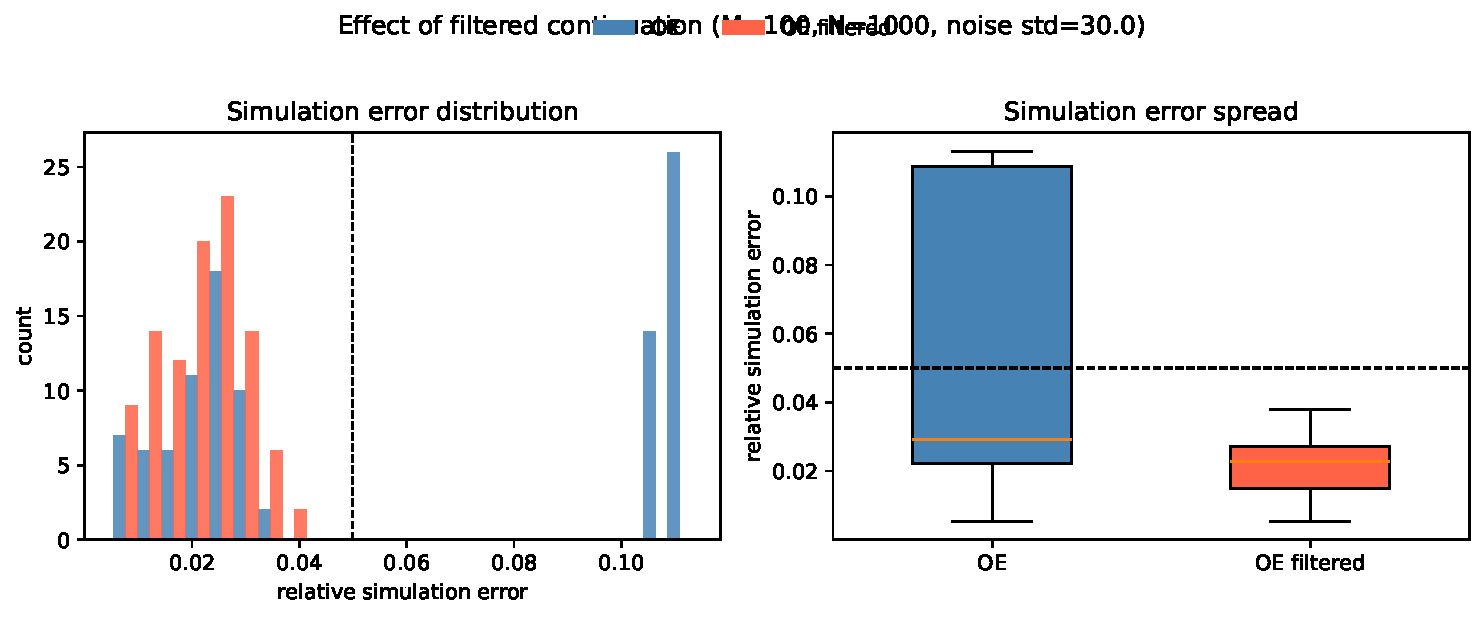
\includegraphics[width=\columnwidth]{experiments/filtered_continuation_oe_errors.pdf}
  \caption{Distribution of the relative simulation error for OE and
           OE filtered on the non-convex problem.
           Dashed line marks the $5\%$ success threshold.}
  \Description{Two panels showing the relative simulation error
    for OE and OE filtered: a histogram comparing their
    distributions, and a boxplot comparing their spreads, with
    a dashed line at the 5 percent success threshold.}
  \label{fig:filtered-errors}
\end{figure}

\section{Conclusion}
\label{sec:conclusion}

\texttt{pysib} is an open-source Python package for parameter
identification of discrete-time SISO systems using classical
polynomial input--output model structures.
It provides a unified interface to ARX, Stieglitz--McBride,
instrumental-variable, correlation, output-error, ARMAX, and
Box--Jenkins estimators, all sharing a common polynomial dictionary
convention so that prediction and simulation can be applied uniformly.

The package makes three main contributions.
First, it fills a gap in the open Python ecosystem by delivering a
focused, well-tested implementation of the key linear and nonlinear
prediction-error estimators, with a simple API and a layered
Python/C architecture.
Second, the nonlinear OE, ARMAX, and BJ estimators use a specialized
low-level optimization core that favors a conservative trajectory of
many small updates over aggressive Newton-type steps; the resulting
workload of cost, gradient, and sensitivity evaluations is made
practical by compiled C extensions and LAPACK linear solvers.
Third, the toolbox provides open implementations of filtered
continuation methods~\cite{eckhard2013input,eckhard2017cost} for the
nonlinear estimators; these methods progressively relax data filters
to drive the estimate toward the original PEM criterion, substantially
reducing sensitivity to local minima.

Numerical experiments show that under noisy data the SM and OE
estimates are centered close to the true parameters, and that the
filtered continuation strategy raises the success rate on a
non-convex OE problem from $60\,\%$ to $100\,\%$.
The complete source code, unit tests, and reproducible drivers are
available through the Collected Algorithms of the ACM and at a
public software archive.

\bibliographystyle{ACM-Reference-Format}
\bibliography{references}

\end{document}
